\documentclass[]{article}
\usepackage{lmodern}
\usepackage{amssymb,amsmath}
\usepackage{ifxetex,ifluatex}
\usepackage{fixltx2e} % provides \textsubscript
\ifnum 0\ifxetex 1\fi\ifluatex 1\fi=0 % if pdftex
  \usepackage[T1]{fontenc}
  \usepackage[utf8]{inputenc}
\else % if luatex or xelatex
  \ifxetex
    \usepackage{mathspec}
  \else
    \usepackage{fontspec}
  \fi
  \defaultfontfeatures{Ligatures=TeX,Scale=MatchLowercase}
\fi
% use upquote if available, for straight quotes in verbatim environments
\IfFileExists{upquote.sty}{\usepackage{upquote}}{}
% use microtype if available
\IfFileExists{microtype.sty}{%
\usepackage{microtype}
\UseMicrotypeSet[protrusion]{basicmath} % disable protrusion for tt fonts
}{}
\usepackage[margin=1in]{geometry}
\usepackage{hyperref}
\hypersetup{unicode=true,
            pdftitle={Advanced Statistical Modelling: Linear Models},
            pdfauthor={Joel Cantero Priego and Ricard Meyerhofer Parra},
            pdfborder={0 0 0},
            breaklinks=true}
\urlstyle{same}  % don't use monospace font for urls
\usepackage{color}
\usepackage{fancyvrb}
\newcommand{\VerbBar}{|}
\newcommand{\VERB}{\Verb[commandchars=\\\{\}]}
\DefineVerbatimEnvironment{Highlighting}{Verbatim}{commandchars=\\\{\}}
% Add ',fontsize=\small' for more characters per line
\usepackage{framed}
\definecolor{shadecolor}{RGB}{248,248,248}
\newenvironment{Shaded}{\begin{snugshade}}{\end{snugshade}}
\newcommand{\KeywordTok}[1]{\textcolor[rgb]{0.13,0.29,0.53}{\textbf{#1}}}
\newcommand{\DataTypeTok}[1]{\textcolor[rgb]{0.13,0.29,0.53}{#1}}
\newcommand{\DecValTok}[1]{\textcolor[rgb]{0.00,0.00,0.81}{#1}}
\newcommand{\BaseNTok}[1]{\textcolor[rgb]{0.00,0.00,0.81}{#1}}
\newcommand{\FloatTok}[1]{\textcolor[rgb]{0.00,0.00,0.81}{#1}}
\newcommand{\ConstantTok}[1]{\textcolor[rgb]{0.00,0.00,0.00}{#1}}
\newcommand{\CharTok}[1]{\textcolor[rgb]{0.31,0.60,0.02}{#1}}
\newcommand{\SpecialCharTok}[1]{\textcolor[rgb]{0.00,0.00,0.00}{#1}}
\newcommand{\StringTok}[1]{\textcolor[rgb]{0.31,0.60,0.02}{#1}}
\newcommand{\VerbatimStringTok}[1]{\textcolor[rgb]{0.31,0.60,0.02}{#1}}
\newcommand{\SpecialStringTok}[1]{\textcolor[rgb]{0.31,0.60,0.02}{#1}}
\newcommand{\ImportTok}[1]{#1}
\newcommand{\CommentTok}[1]{\textcolor[rgb]{0.56,0.35,0.01}{\textit{#1}}}
\newcommand{\DocumentationTok}[1]{\textcolor[rgb]{0.56,0.35,0.01}{\textbf{\textit{#1}}}}
\newcommand{\AnnotationTok}[1]{\textcolor[rgb]{0.56,0.35,0.01}{\textbf{\textit{#1}}}}
\newcommand{\CommentVarTok}[1]{\textcolor[rgb]{0.56,0.35,0.01}{\textbf{\textit{#1}}}}
\newcommand{\OtherTok}[1]{\textcolor[rgb]{0.56,0.35,0.01}{#1}}
\newcommand{\FunctionTok}[1]{\textcolor[rgb]{0.00,0.00,0.00}{#1}}
\newcommand{\VariableTok}[1]{\textcolor[rgb]{0.00,0.00,0.00}{#1}}
\newcommand{\ControlFlowTok}[1]{\textcolor[rgb]{0.13,0.29,0.53}{\textbf{#1}}}
\newcommand{\OperatorTok}[1]{\textcolor[rgb]{0.81,0.36,0.00}{\textbf{#1}}}
\newcommand{\BuiltInTok}[1]{#1}
\newcommand{\ExtensionTok}[1]{#1}
\newcommand{\PreprocessorTok}[1]{\textcolor[rgb]{0.56,0.35,0.01}{\textit{#1}}}
\newcommand{\AttributeTok}[1]{\textcolor[rgb]{0.77,0.63,0.00}{#1}}
\newcommand{\RegionMarkerTok}[1]{#1}
\newcommand{\InformationTok}[1]{\textcolor[rgb]{0.56,0.35,0.01}{\textbf{\textit{#1}}}}
\newcommand{\WarningTok}[1]{\textcolor[rgb]{0.56,0.35,0.01}{\textbf{\textit{#1}}}}
\newcommand{\AlertTok}[1]{\textcolor[rgb]{0.94,0.16,0.16}{#1}}
\newcommand{\ErrorTok}[1]{\textcolor[rgb]{0.64,0.00,0.00}{\textbf{#1}}}
\newcommand{\NormalTok}[1]{#1}
\usepackage{longtable,booktabs}
\usepackage{graphicx,grffile}
\makeatletter
\def\maxwidth{\ifdim\Gin@nat@width>\linewidth\linewidth\else\Gin@nat@width\fi}
\def\maxheight{\ifdim\Gin@nat@height>\textheight\textheight\else\Gin@nat@height\fi}
\makeatother
% Scale images if necessary, so that they will not overflow the page
% margins by default, and it is still possible to overwrite the defaults
% using explicit options in \includegraphics[width, height, ...]{}
\setkeys{Gin}{width=\maxwidth,height=\maxheight,keepaspectratio}
\IfFileExists{parskip.sty}{%
\usepackage{parskip}
}{% else
\setlength{\parindent}{0pt}
\setlength{\parskip}{6pt plus 2pt minus 1pt}
}
\setlength{\emergencystretch}{3em}  % prevent overfull lines
\providecommand{\tightlist}{%
  \setlength{\itemsep}{0pt}\setlength{\parskip}{0pt}}
\setcounter{secnumdepth}{0}
% Redefines (sub)paragraphs to behave more like sections
\ifx\paragraph\undefined\else
\let\oldparagraph\paragraph
\renewcommand{\paragraph}[1]{\oldparagraph{#1}\mbox{}}
\fi
\ifx\subparagraph\undefined\else
\let\oldsubparagraph\subparagraph
\renewcommand{\subparagraph}[1]{\oldsubparagraph{#1}\mbox{}}
\fi

%%% Use protect on footnotes to avoid problems with footnotes in titles
\let\rmarkdownfootnote\footnote%
\def\footnote{\protect\rmarkdownfootnote}

%%% Change title format to be more compact
\usepackage{titling}

% Create subtitle command for use in maketitle
\newcommand{\subtitle}[1]{
  \posttitle{
    \begin{center}\large#1\end{center}
    }
}

\setlength{\droptitle}{-2em}

  \title{Advanced Statistical Modelling: Linear Models}
    \pretitle{\vspace{\droptitle}\centering\huge}
  \posttitle{\par}
    \author{Joel Cantero Priego and Ricard Meyerhofer Parra}
    \preauthor{\centering\large\emph}
  \postauthor{\par}
      \predate{\centering\large\emph}
  \postdate{\par}
    \date{12/10/2019}

\usepackage{booktabs}
\usepackage{longtable}
\usepackage{array}
\usepackage{multirow}
\usepackage{wrapfig}
\usepackage{float}
\usepackage{colortbl}
\usepackage{pdflscape}
\usepackage{tabu}
\usepackage{threeparttable}
\usepackage{threeparttablex}
\usepackage[normalem]{ulem}
\usepackage{makecell}
\usepackage{xcolor}

\begin{document}
\maketitle

\subsection{Introduction}\label{introduction}

In this assignment, we are going to use the IMDB dataset. This IMDB
dataset, contains information of 940 films released between 2000 and
2016. The data has been obtained from the IMDB's webpage. The following
is a list where we can see all the variables of the dataset:

\begin{longtable}[]{@{}ccc@{}}
\toprule
Variable name & Description & Values\tabularnewline
\midrule
\endhead
movietitle & Director of the given title & String\tabularnewline
gross & Gross in dollars & Integer\tabularnewline
budget & Budget in dollars & Integer\tabularnewline
duration & Film duration in minutes & Integer\tabularnewline
titleyear & The release year of the title & Integer\tabularnewline
directorfl & Director Facebook likes & Integer\tabularnewline
actor1fl & Actor 1 Facebook likes & Integer\tabularnewline
actor2fl & Actor 2 Facebook likes & Integer\tabularnewline
actor3fl & Actor 3 Facebook likes & Integer\tabularnewline
castfl & Cast Facebook likes & Integer\tabularnewline
facenumber\_in\_poster & Number of faces that appears in the poster &
Integer\tabularnewline
genre & Genre film & Action/Comedy/Drama/Terror\tabularnewline
\bottomrule
\end{longtable}

As we can see we have that all our variables are numerical in exception
genre. This dataset is complete which means that it has no missing
values. However, this does not imply that there are no outliers.

As required in the assignment, we are going to create a categorical
variable: yearcat which is the categorical substitution of titleyear
with 3 levels: 2000-2005, 2006-2010 and 2011-2016. Therefore, we will
have two categorical variables (genre and titleyear).

\begin{Shaded}
\begin{Highlighting}[]
\NormalTok{dataset}\OperatorTok{$}\NormalTok{yearcat<-}\KeywordTok{cut}\NormalTok{(dataset}\OperatorTok{$}\NormalTok{titleyear, }\KeywordTok{c}\NormalTok{(}\DecValTok{2000}\NormalTok{,}\DecValTok{2005}\NormalTok{,}\DecValTok{2010}\NormalTok{,}\DecValTok{2016}\NormalTok{), }
                   \DataTypeTok{include.lowest =} \OtherTok{TRUE}\NormalTok{, }
                   \DataTypeTok{labels=}\KeywordTok{c}\NormalTok{(}\StringTok{"2000-2005"}\NormalTok{, }\StringTok{"2006-2010"}\NormalTok{, }\StringTok{"2011-2016"}\NormalTok{))}
\end{Highlighting}
\end{Shaded}

\subsection{Exploratory Data Analysis}\label{exploratory-data-analysis}

In this section we are going to focus in explaining the most interesting
conclusions of our data, perform an univariate and multivariate analysis
of the variables in order to find outliers and see the relationship and
structure of the dataset variables.

\subsubsection{Missing values remark}\label{missing-values-remark}

As previously mentioned, there are no missing values. However, we can
see that there are some 0 values in directorfl column but we can
interpret them as they do not own any Facebook page.

\begin{Shaded}
\begin{Highlighting}[]
\KeywordTok{length}\NormalTok{(}\KeywordTok{which}\NormalTok{(dataset}\OperatorTok{$}\NormalTok{directorfl}\OperatorTok{==}\DecValTok{0}\NormalTok{))}\OperatorTok{/}\KeywordTok{length}\NormalTok{(dataset}\OperatorTok{$}\NormalTok{directorfl)}
\end{Highlighting}
\end{Shaded}

\begin{verbatim}
## [1] 0.1638298
\end{verbatim}

\subsubsection{plotting stuffs:}\label{plotting-stuffs}

\subsubsection{Univariate analysis}\label{univariate-analysis}

For univariate analysis, histograms and box plot were obtained for the
numerical variables and bar charts were generated for the categorical
variables. These are the results obtained:

We can see usual values for the Budget, with a mean of 40,484,550\$.

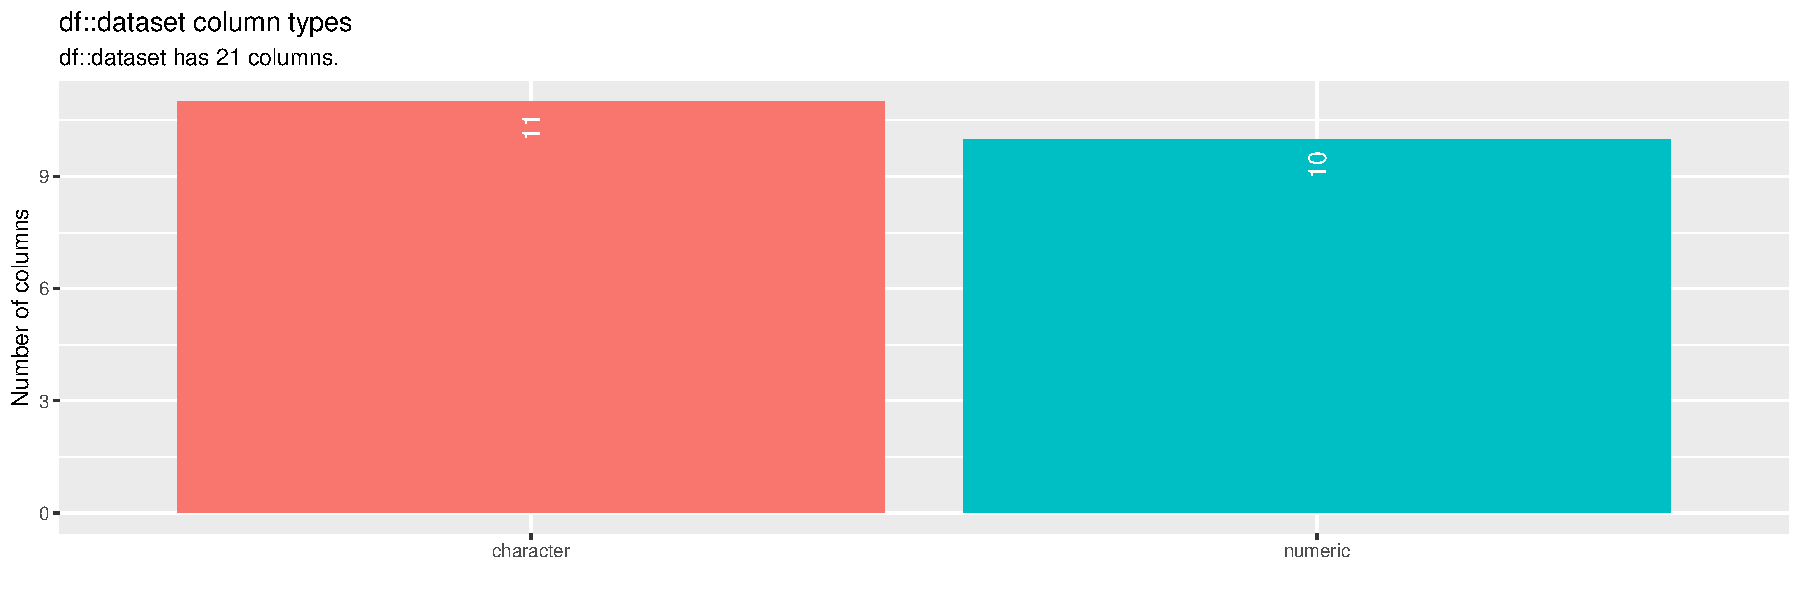
\includegraphics{deliverable_files/figure-latex/unnamed-chunk-3-1.pdf}

In duration film, we see that there is a certain tendency to normality
centred around 100 minutes, we consider it as usual. There is a strange
observation of 280 minutes for ``Gods and General'' film. After check
it, we can say that it is not an error but an extrem value.

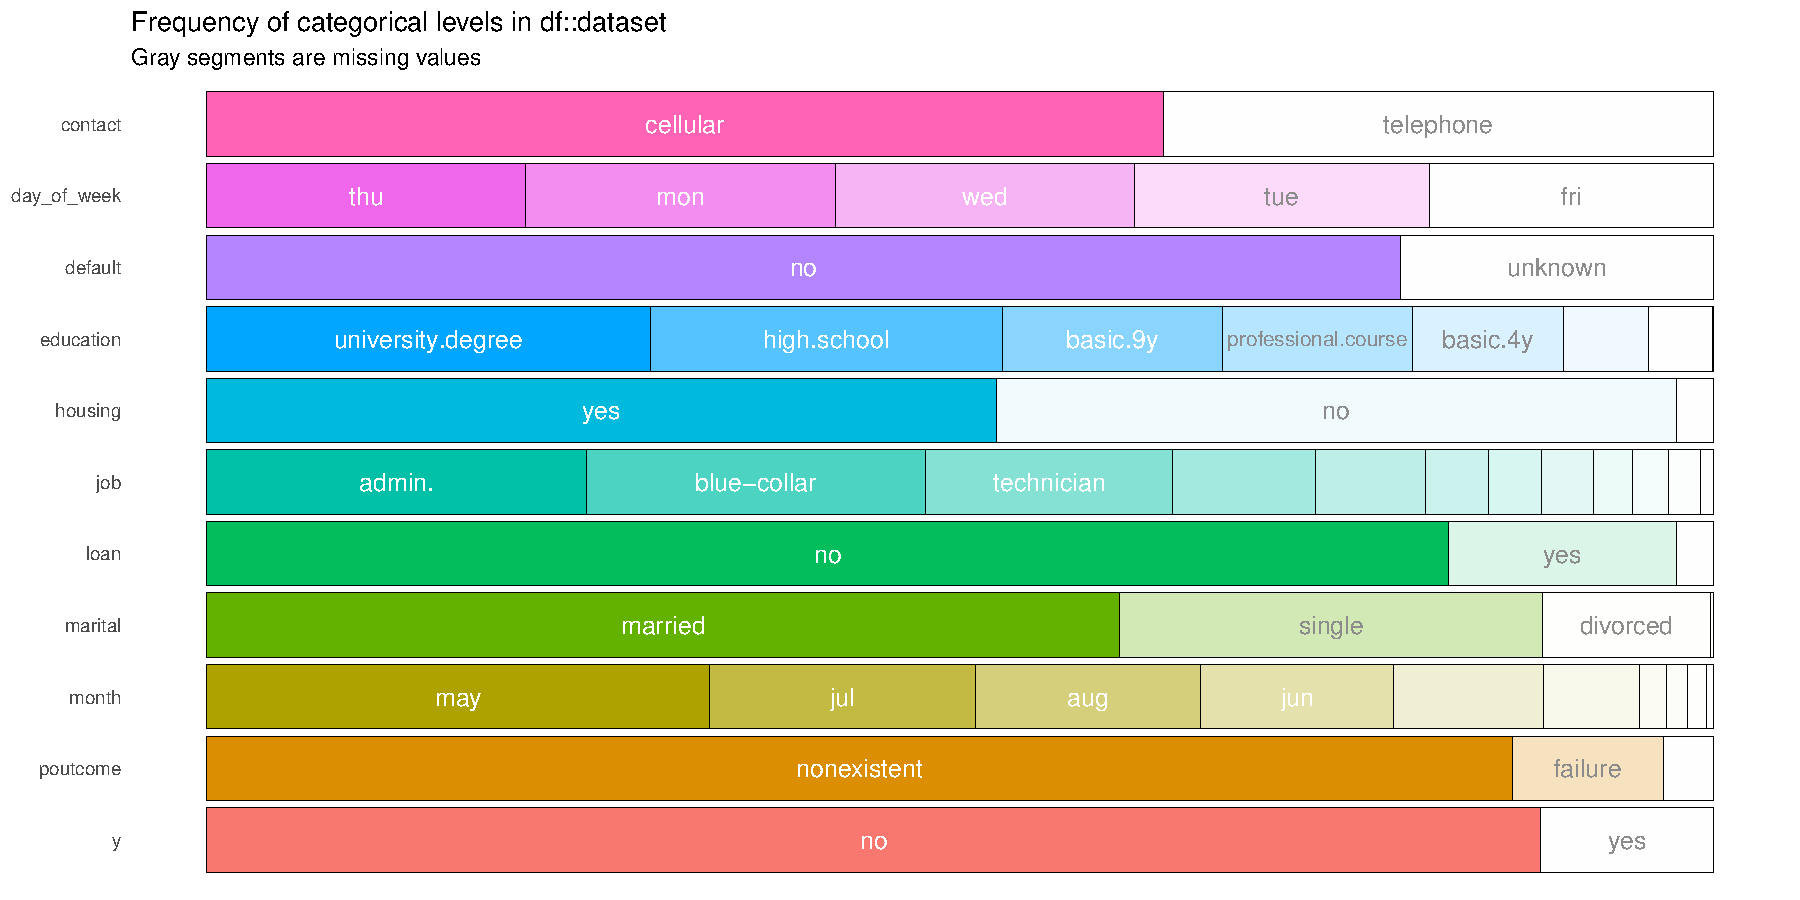
\includegraphics{deliverable_files/figure-latex/unnamed-chunk-4-1.pdf}

No problems for year, there is a certain expected balanced in years
proportion.

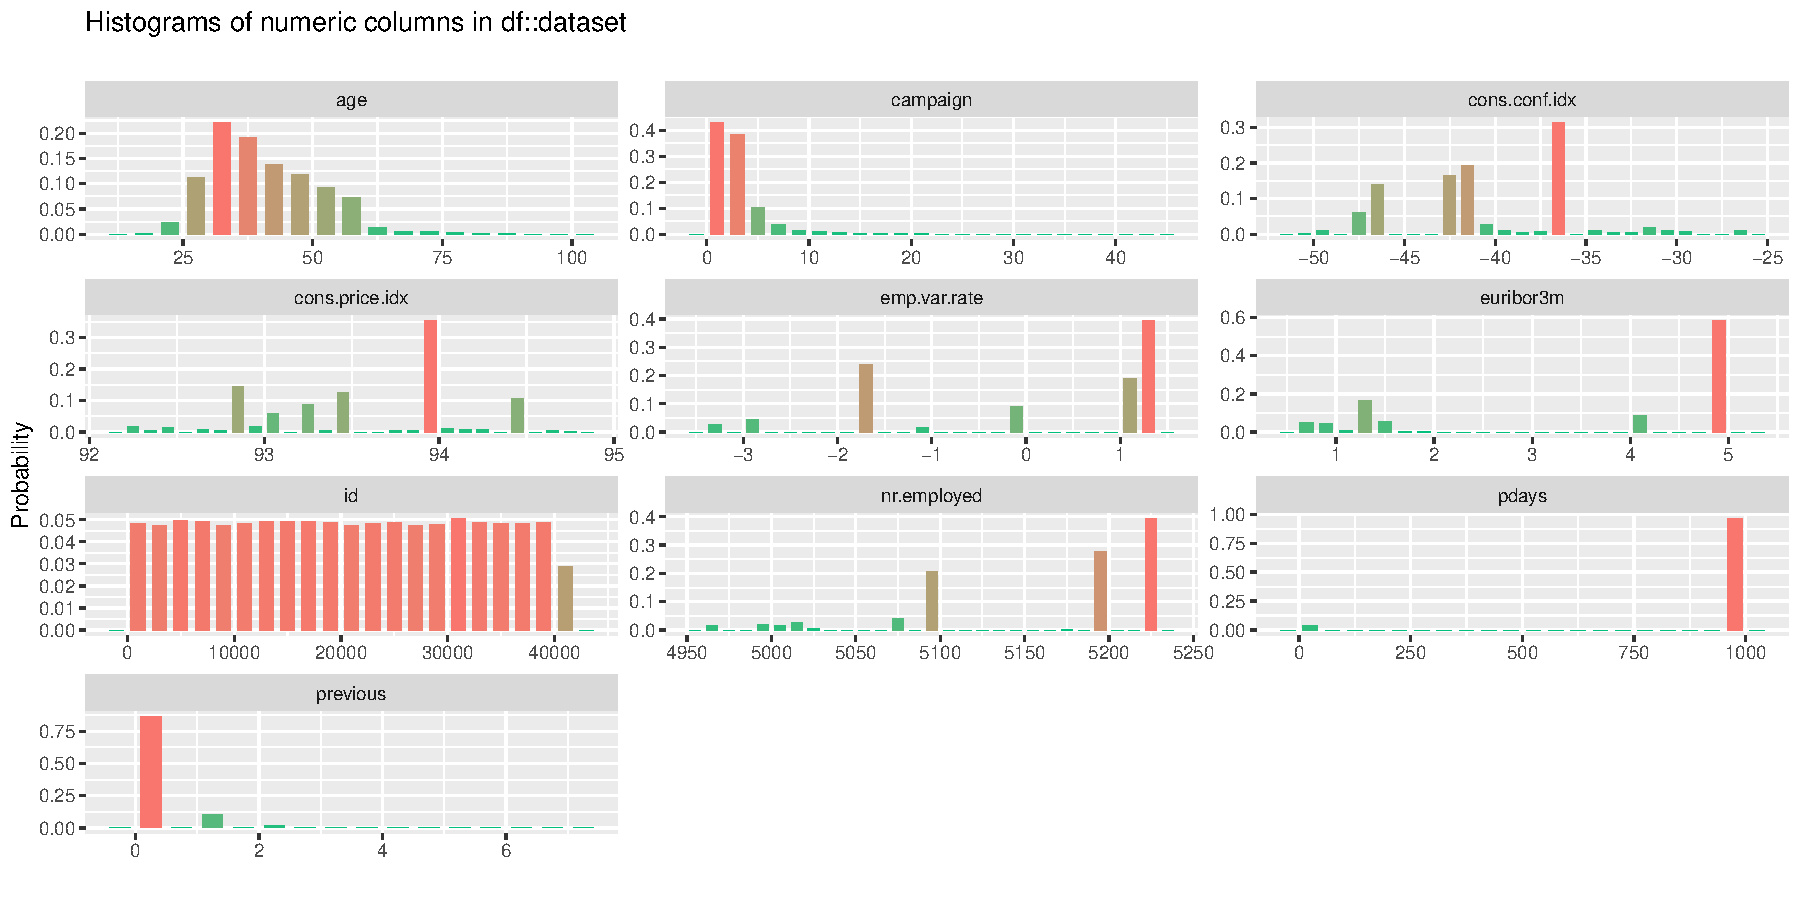
\includegraphics{deliverable_files/figure-latex/unnamed-chunk-5-1.pdf}

In Director Facebook likes, we see that there is a value which appears
in the majority of the cases: In this case, is the 0 value. Apart from
this zero value, we see that small number of likes are more common than
medium or higher number of likes.

\includegraphics{deliverable_files/figure-latex/unnamed-chunk-6-1.pdf}

In face number in film poster, the mean is about 1,6 faces and we can
observe an extrem value of 31 in ``The Master''. We can say once again
that it is not an error but an extrem value.

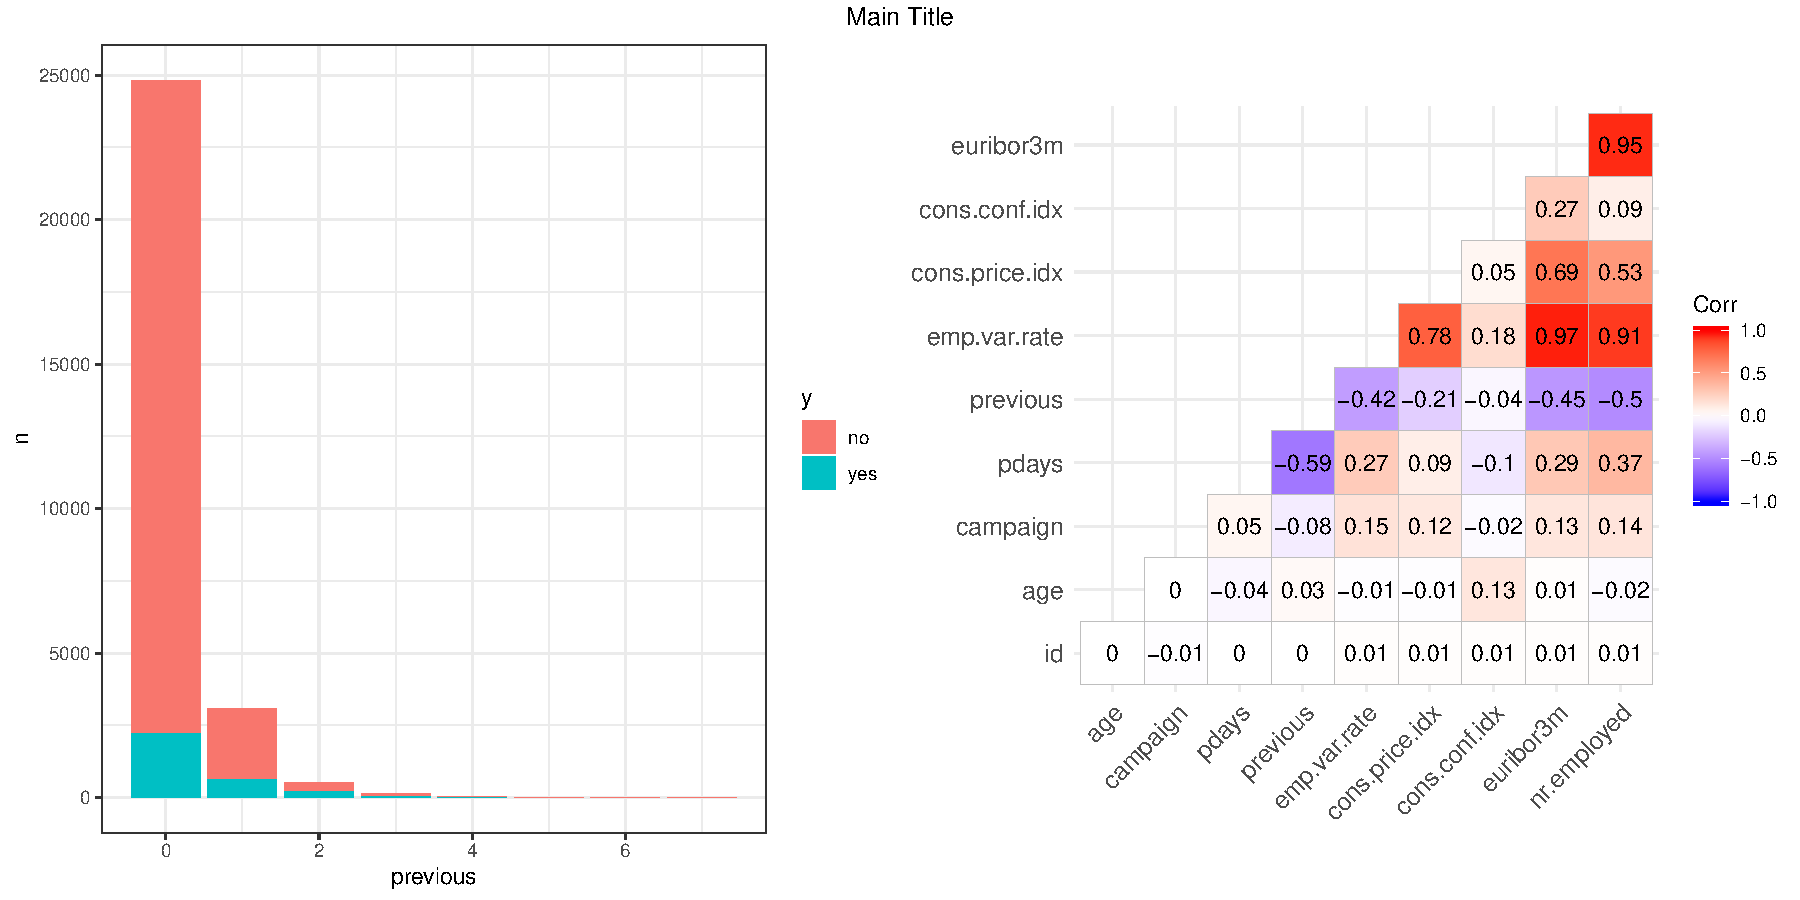
\includegraphics{deliverable_files/figure-latex/unnamed-chunk-7-1.pdf}

In genre film we can observe that there are more comedy and drama films
than action and terror films.

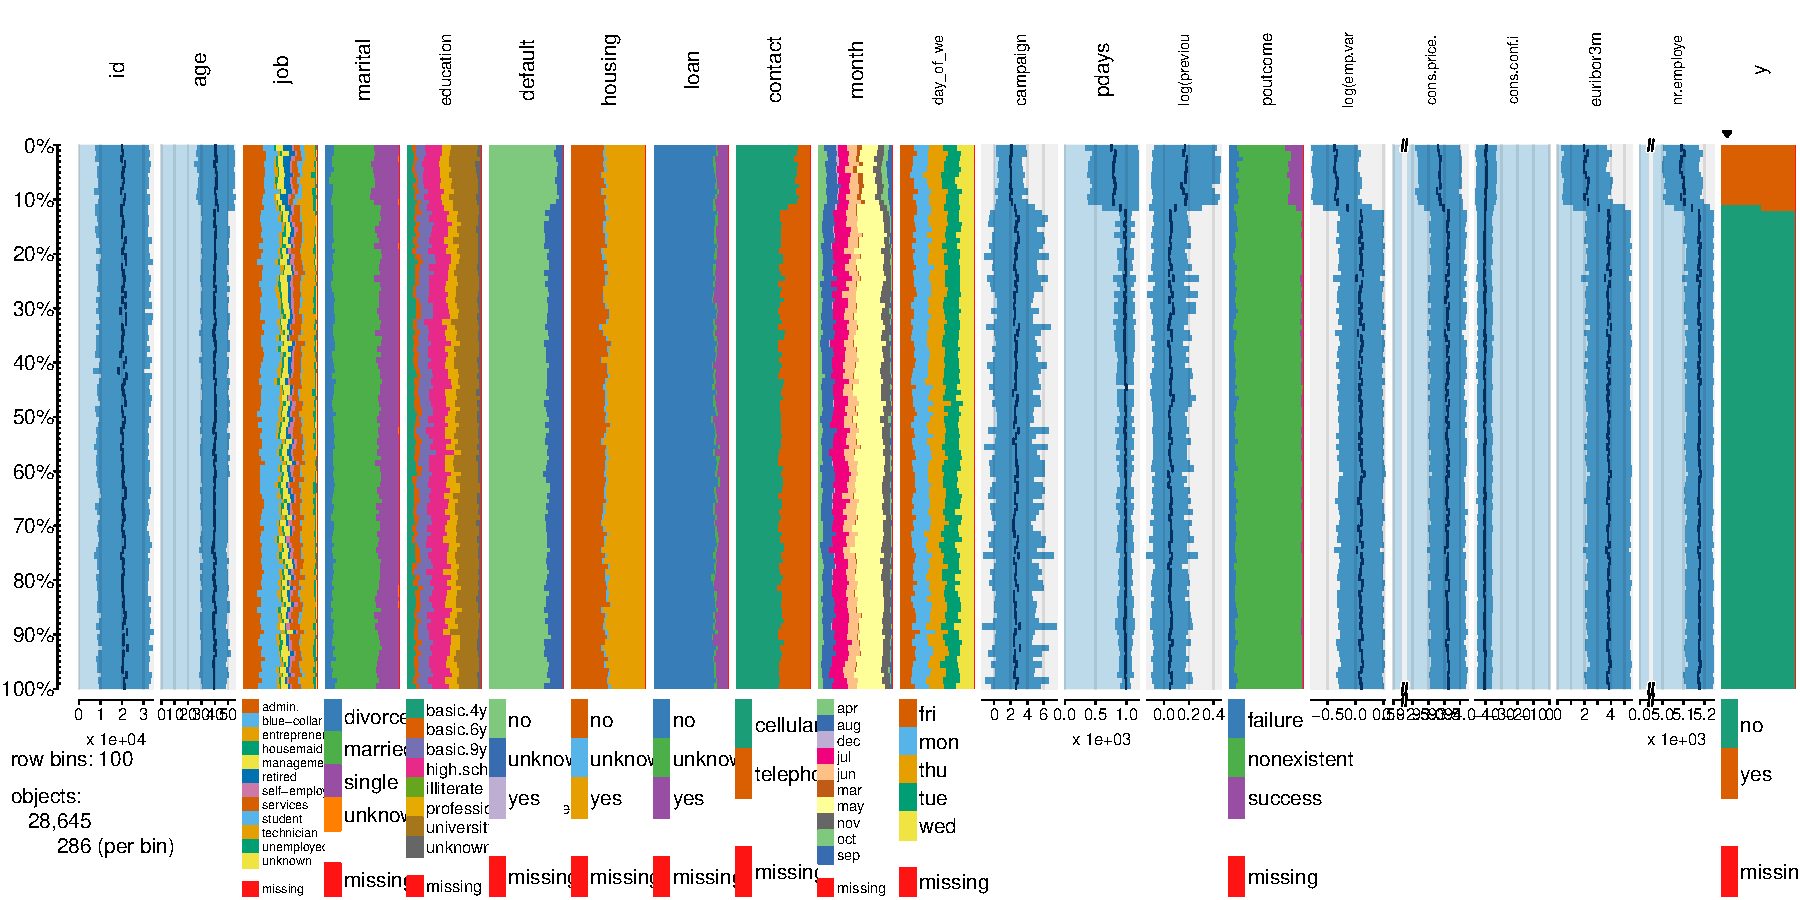
\includegraphics{deliverable_files/figure-latex/unnamed-chunk-8-1.pdf}

Thanks to cross-correlation matrix, we can see that there is a positive
correlation between gross and budget variable (0,729). On the other hand
there is positive correlation between Cast Facebook Likes and Actor
Facebook likes.

\includegraphics{deliverable_files/figure-latex/pressure-1.pdf}

\begin{table}[H]
\centering
\resizebox{\linewidth}{!}{
\begin{tabular}{lrrrrrrrrr}
\toprule
  & gross & budget & duration & directorfl & actor1fl & actor2fl & actor3fl & castfl & facenumber\_in\_poster\\
\midrule
gross & 1.0000000 & 0.7295407 & 0.4169113 & 0.1135821 & 0.1203821 & 0.2516909 & 0.3897209 & 0.2117592 & 0.0029669\\
budget & 0.7295407 & 1.0000000 & 0.4807725 & 0.1185898 & 0.1384697 & 0.2587875 & 0.3404662 & 0.2198807 & -0.0065147\\
duration & 0.4169113 & 0.4807725 & 1.0000000 & 0.2152645 & 0.0649505 & 0.1288276 & 0.1809332 & 0.1070346 & -0.0123550\\
directorfl & 0.1135821 & 0.1185898 & 0.2152645 & 1.0000000 & 0.0660325 & 0.0940824 & 0.0453623 & 0.0825869 & -0.0843436\\
actor1fl & 0.1203821 & 0.1384697 & 0.0649505 & 0.0660325 & 1.0000000 & 0.3491797 & 0.2377791 & 0.9618000 & 0.0551944\\
\addlinespace
actor2fl & 0.2516909 & 0.2587875 & 0.1288276 & 0.0940824 & 0.3491797 & 1.0000000 & 0.4591963 & 0.5725142 & 0.0258751\\
actor3fl & 0.3897209 & 0.3404662 & 0.1809332 & 0.0453623 & 0.2377791 & 0.4591963 & 1.0000000 & 0.4160769 & 0.0847390\\
castfl & 0.2117592 & 0.2198807 & 0.1070346 & 0.0825869 & 0.9618000 & 0.5725142 & 0.4160769 & 1.0000000 & 0.0650337\\
facenumber\_in\_poster & 0.0029669 & -0.0065147 & -0.0123550 & -0.0843436 & 0.0551944 & 0.0258751 & 0.0847390 & 0.0650337 & 1.0000000\\
\bottomrule
\end{tabular}}
\end{table}

\begin{Shaded}
\begin{Highlighting}[]
\CommentTok{# Gross variable exploration}
\KeywordTok{summary}\NormalTok{(dataset}\OperatorTok{$}\NormalTok{gross)}
\end{Highlighting}
\end{Shaded}

\begin{verbatim}
##      Min.   1st Qu.    Median      Mean   3rd Qu.      Max. 
##      3330  11816543  33428175  57813237  70756664 760505847
\end{verbatim}

\begin{Shaded}
\begin{Highlighting}[]
\KeywordTok{boxplot}\NormalTok{(dataset}\OperatorTok{$}\NormalTok{gross)}
\end{Highlighting}
\end{Shaded}

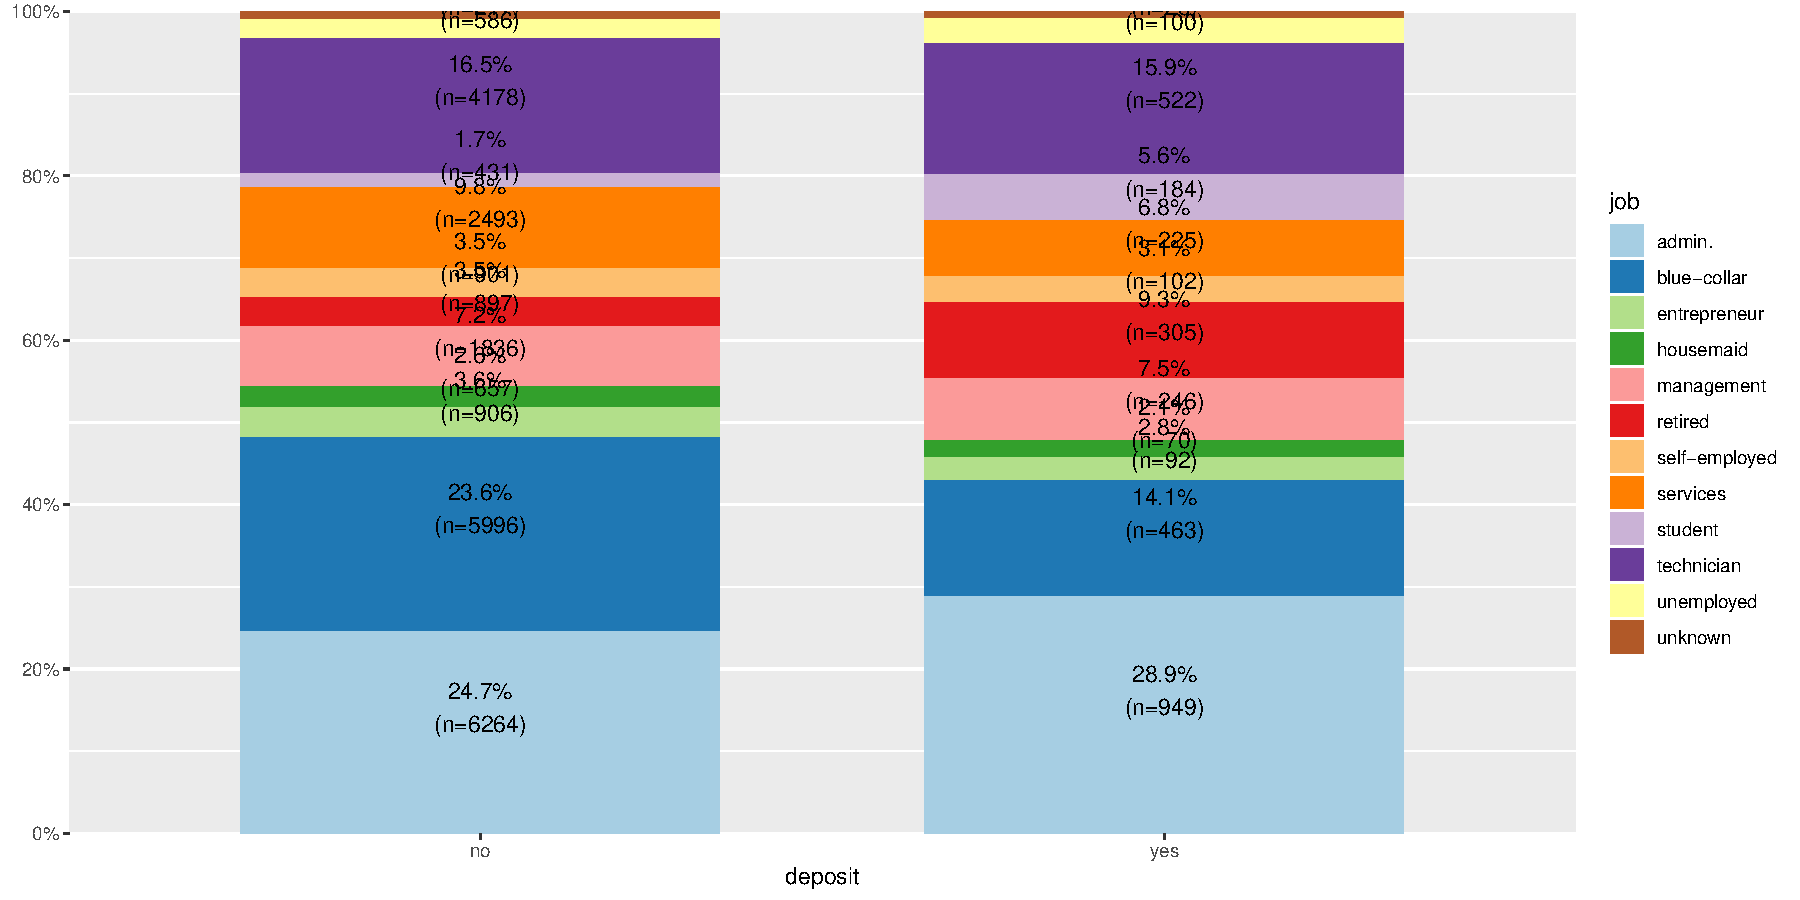
\includegraphics{deliverable_files/figure-latex/unnamed-chunk-9-1.pdf}

\begin{Shaded}
\begin{Highlighting}[]
\KeywordTok{plot}\NormalTok{(}\KeywordTok{density}\NormalTok{(dataset}\OperatorTok{$}\NormalTok{gross), }\DataTypeTok{main=}\StringTok{"Density plot of gross"}\NormalTok{)}
\end{Highlighting}
\end{Shaded}

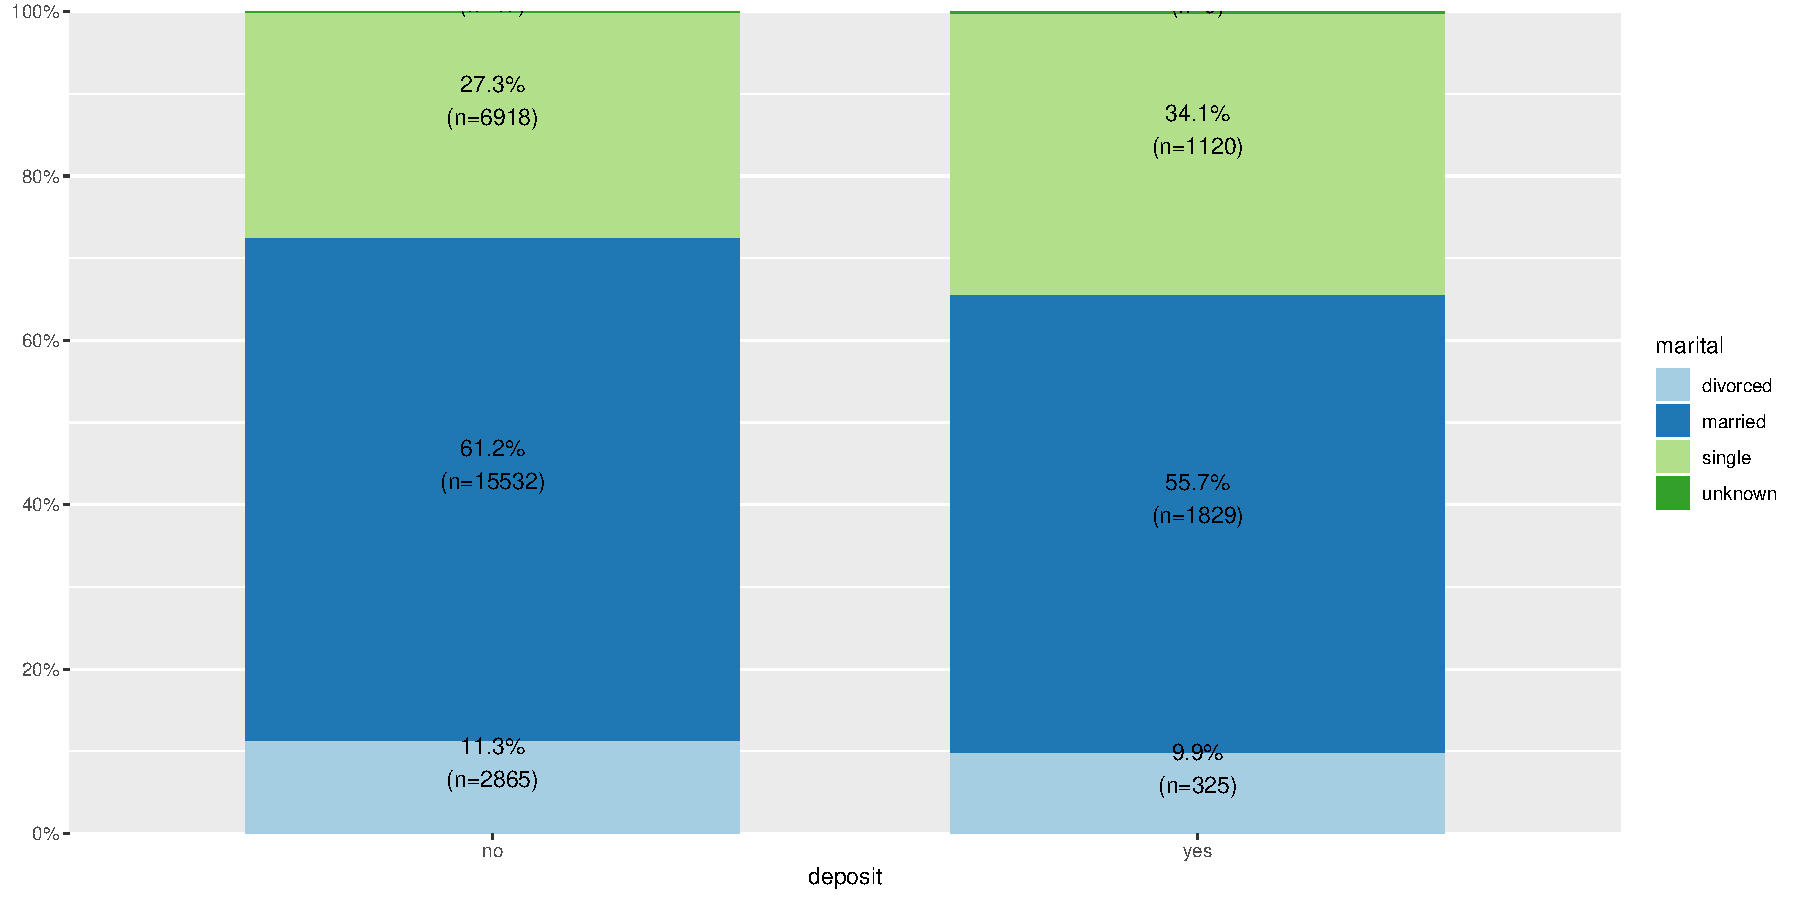
\includegraphics{deliverable_files/figure-latex/unnamed-chunk-9-2.pdf}

\begin{Shaded}
\begin{Highlighting}[]
\CommentTok{#Histogram/Density Function}
\KeywordTok{hist}\NormalTok{(dataset}\OperatorTok{$}\NormalTok{gross)}
\end{Highlighting}
\end{Shaded}

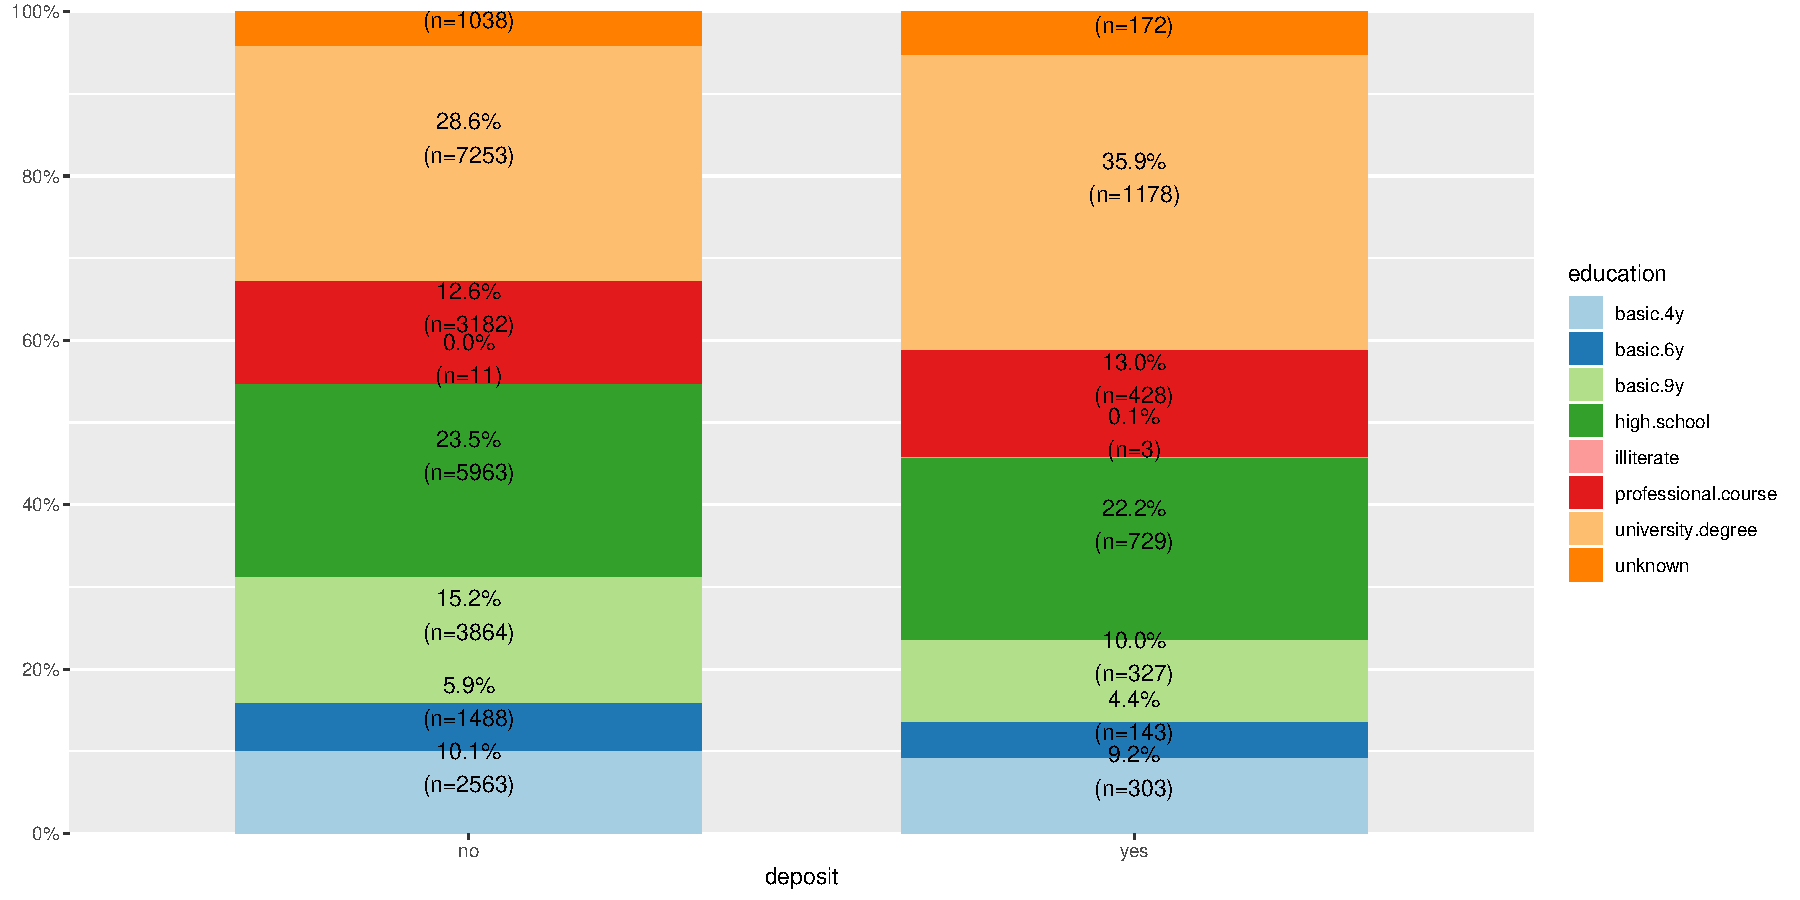
\includegraphics{deliverable_files/figure-latex/unnamed-chunk-9-3.pdf}

\begin{Shaded}
\begin{Highlighting}[]
\KeywordTok{cat}\NormalTok{(}\StringTok{"Sample Mean}\CharTok{\textbackslash{}n}\StringTok{"}\NormalTok{)}
\end{Highlighting}
\end{Shaded}

\begin{verbatim}
## Sample Mean
\end{verbatim}

\begin{Shaded}
\begin{Highlighting}[]
\NormalTok{(}\DataTypeTok{m=}\KeywordTok{mean}\NormalTok{(dataset}\OperatorTok{$}\NormalTok{gross))}
\end{Highlighting}
\end{Shaded}

\begin{verbatim}
## [1] 57813237
\end{verbatim}

\begin{Shaded}
\begin{Highlighting}[]
\KeywordTok{cat}\NormalTok{(}\StringTok{"Sample Sd}\CharTok{\textbackslash{}n}\StringTok{"}\NormalTok{)}
\end{Highlighting}
\end{Shaded}

\begin{verbatim}
## Sample Sd
\end{verbatim}

\begin{Shaded}
\begin{Highlighting}[]
\NormalTok{(}\DataTypeTok{s=}\KeywordTok{sd}\NormalTok{(dataset}\OperatorTok{$}\NormalTok{gross))}
\end{Highlighting}
\end{Shaded}

\begin{verbatim}
## [1] 77110518
\end{verbatim}

\begin{Shaded}
\begin{Highlighting}[]
\KeywordTok{cat}\NormalTok{(}\StringTok{"LogLik}\CharTok{\textbackslash{}n}\StringTok{"}\NormalTok{)}
\end{Highlighting}
\end{Shaded}

\begin{verbatim}
## LogLik
\end{verbatim}

\begin{Shaded}
\begin{Highlighting}[]
\NormalTok{(}\DataTypeTok{loglik=}\KeywordTok{sum}\NormalTok{(}\KeywordTok{log}\NormalTok{(}\KeywordTok{dnorm}\NormalTok{(dataset}\OperatorTok{$}\NormalTok{gross,}\DataTypeTok{mean=}\KeywordTok{mean}\NormalTok{(dataset}\OperatorTok{$}\NormalTok{gross),}\DataTypeTok{sd=}\KeywordTok{sd}\NormalTok{(dataset}\OperatorTok{$}\NormalTok{gross)))))}
\end{Highlighting}
\end{Shaded}

\begin{verbatim}
## [1] -18404.41
\end{verbatim}

\begin{Shaded}
\begin{Highlighting}[]
\KeywordTok{cat}\NormalTok{(}\StringTok{"AIC}\CharTok{\textbackslash{}n}\StringTok{"}\NormalTok{)}
\end{Highlighting}
\end{Shaded}

\begin{verbatim}
## AIC
\end{verbatim}

\begin{Shaded}
\begin{Highlighting}[]
\NormalTok{(}\DataTypeTok{AIC=}\OperatorTok{-}\DecValTok{2}\OperatorTok{*}\NormalTok{loglik}\OperatorTok{+}\DecValTok{2}\OperatorTok{*}\DecValTok{2}\NormalTok{)}
\end{Highlighting}
\end{Shaded}

\begin{verbatim}
## [1] 36812.81
\end{verbatim}

\begin{Shaded}
\begin{Highlighting}[]
\CommentTok{#Plot Quantiles-Quantiles (Empirical-Theorical)}
\KeywordTok{qqplot}\NormalTok{(}\KeywordTok{qnorm}\NormalTok{(}\KeywordTok{ppoints}\NormalTok{(}\DecValTok{500}\NormalTok{),}\DataTypeTok{mean=}\NormalTok{m,}\DataTypeTok{sd=}\NormalTok{s),dataset}\OperatorTok{$}\NormalTok{gross)}
\end{Highlighting}
\end{Shaded}

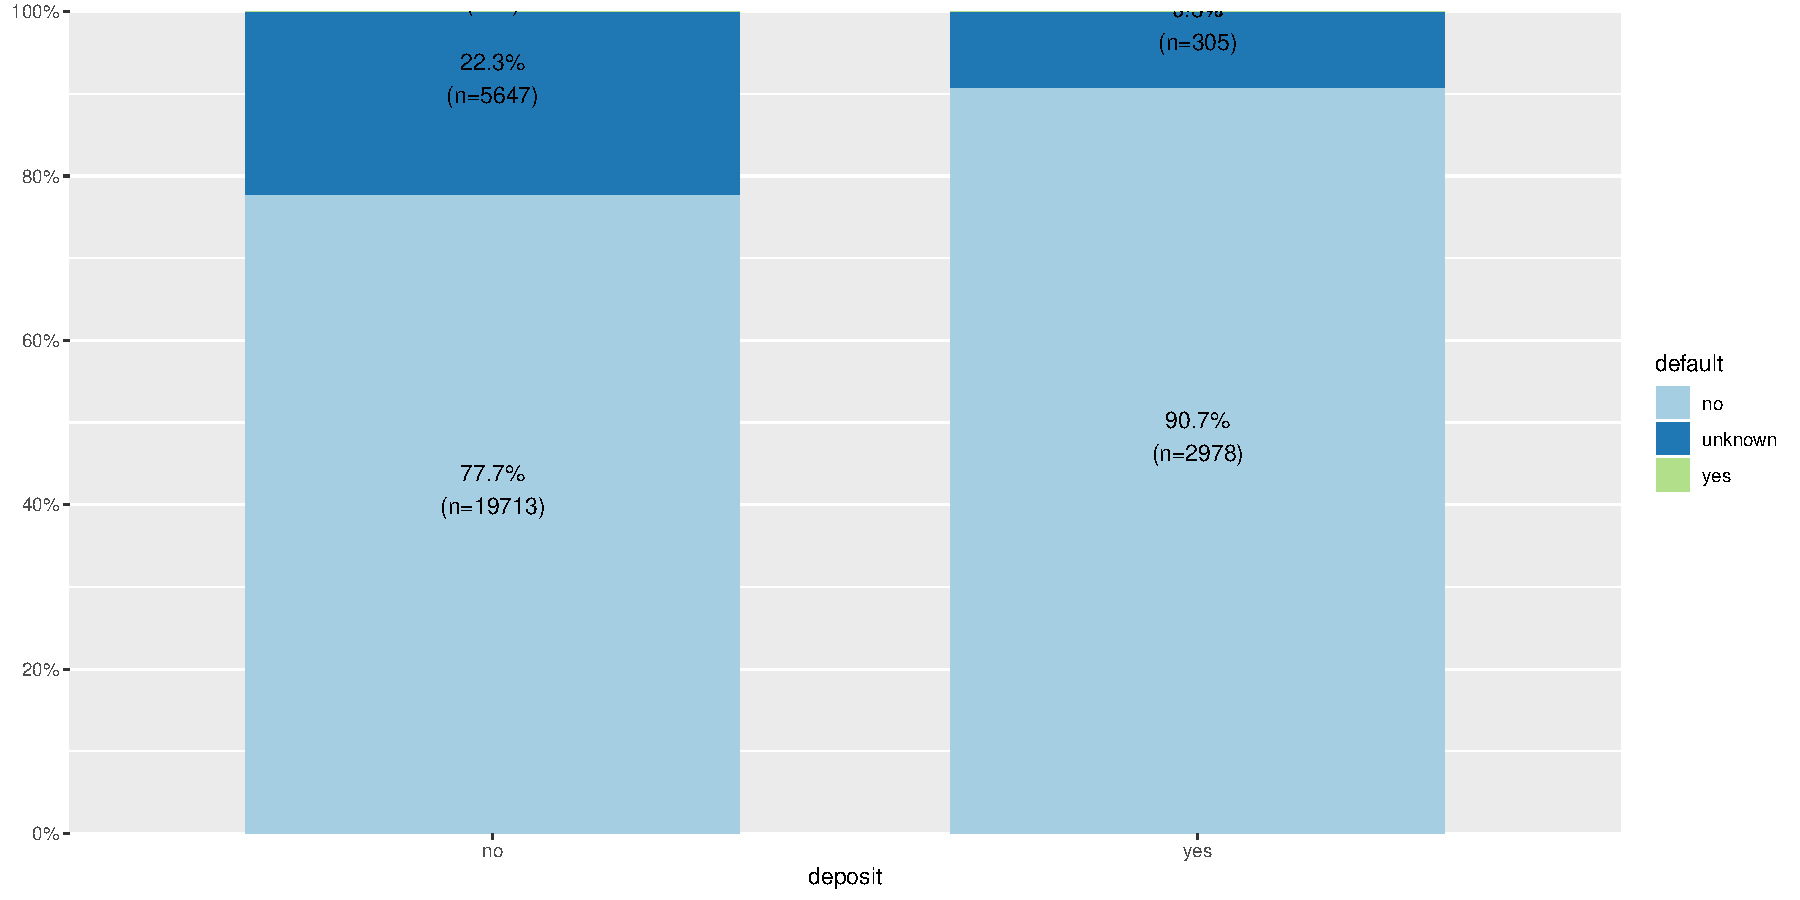
\includegraphics{deliverable_files/figure-latex/unnamed-chunk-9-4.pdf}

\begin{Shaded}
\begin{Highlighting}[]
\KeywordTok{qqnorm}\NormalTok{(dataset}\OperatorTok{$}\NormalTok{gross)}
\end{Highlighting}
\end{Shaded}

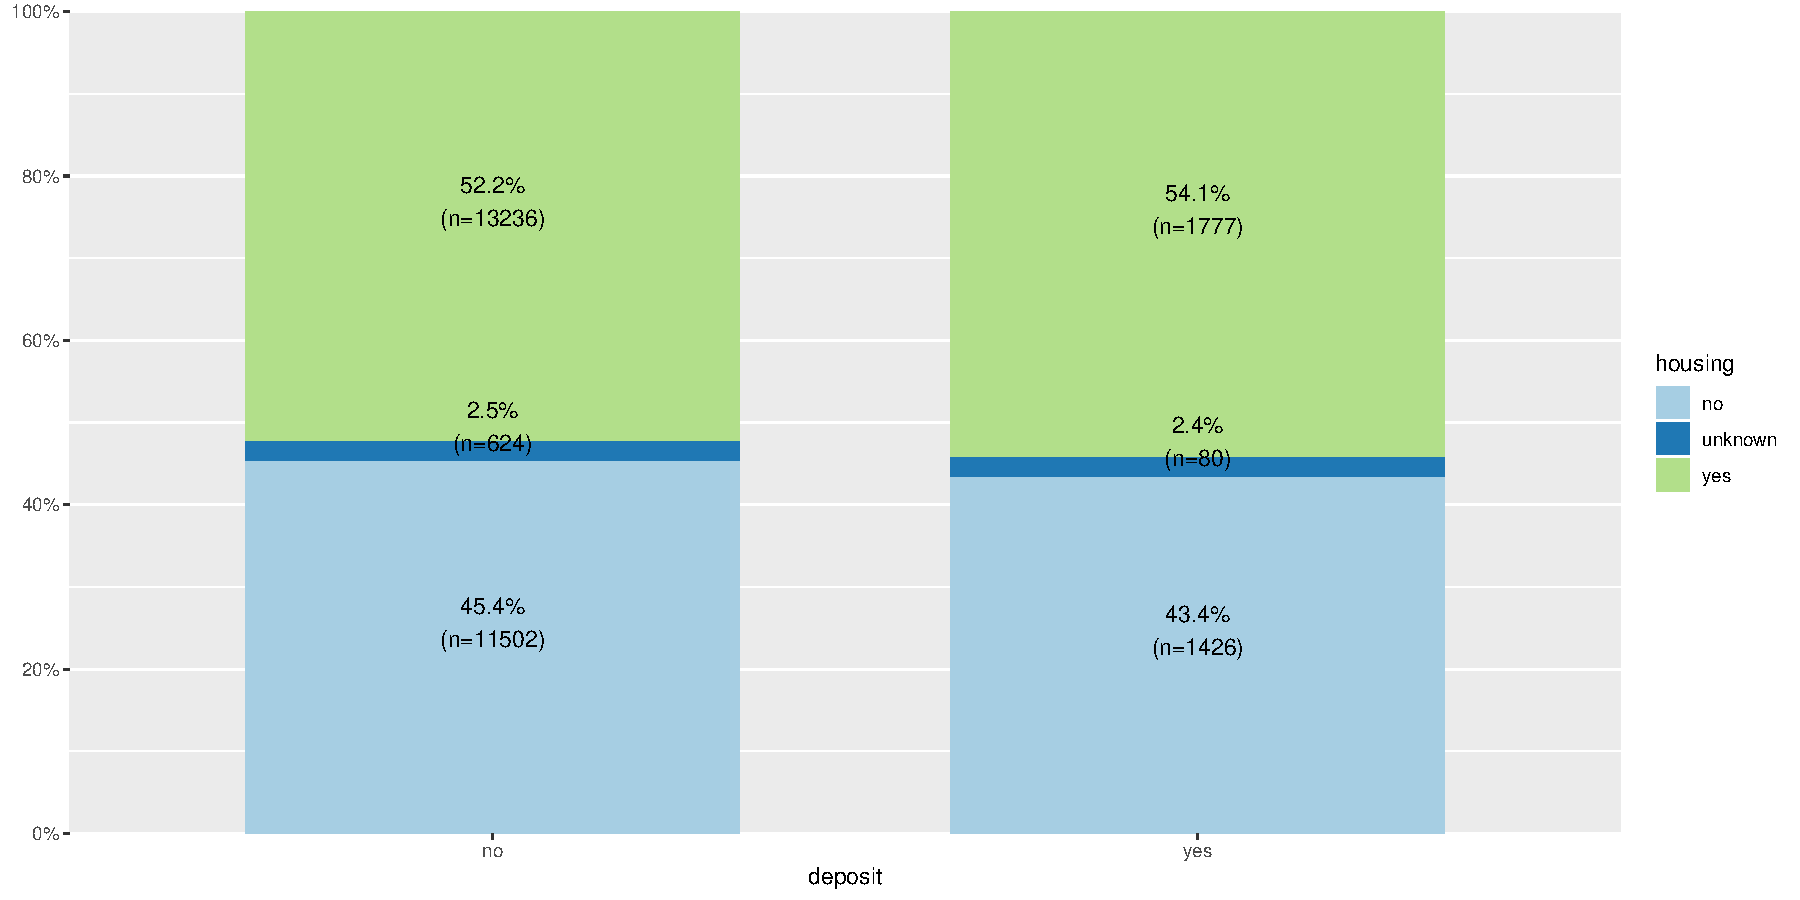
\includegraphics{deliverable_files/figure-latex/unnamed-chunk-9-5.pdf}

In gross, our target variable, we see that there is a certain tendency
to normality centred around 60.000.000\$,

The highest grossing film is Avatar (760,505,847\$) and the lowest is Mi
America (3330\$).

\subsection{Fitting the complete
model}\label{fitting-the-complete-model}

\begin{Shaded}
\begin{Highlighting}[]
\CommentTok{#Linear Regression}
\KeywordTok{summary}\NormalTok{(m1<-}\KeywordTok{lm}\NormalTok{(gross }\OperatorTok{~}\StringTok{ }\NormalTok{budget }\OperatorTok{+}\StringTok{ }\NormalTok{duration }\OperatorTok{+}\StringTok{ }\NormalTok{titleyear }\OperatorTok{+}\StringTok{ }\NormalTok{directorfl }\OperatorTok{+}\StringTok{ }\NormalTok{actor1fl }\OperatorTok{+}\StringTok{ }\NormalTok{actor2fl }\OperatorTok{+}\StringTok{ }\NormalTok{actor3fl }\OperatorTok{+}\StringTok{ }\NormalTok{castfl }\OperatorTok{+}\StringTok{ }\NormalTok{facenumber_in_poster }\OperatorTok{+}\StringTok{ }\NormalTok{genre, dataset))}
\end{Highlighting}
\end{Shaded}

\begin{verbatim}
## 
## Call:
## lm(formula = gross ~ budget + duration + titleyear + directorfl + 
##     actor1fl + actor2fl + actor3fl + castfl + facenumber_in_poster + 
##     genre, data = dataset)
## 
## Residuals:
##        Min         1Q     Median         3Q        Max 
## -190336090  -24098803   -6743291   16624251  481357273 
## 
## Coefficients:
##                        Estimate Std. Error t value Pr(>|t|)    
## (Intercept)           5.583e+07  7.205e+08   0.077  0.93826    
## budget                9.590e-01  5.812e-02  16.500  < 2e-16 ***
## duration              5.068e+05  1.054e+05   4.808 1.78e-06 ***
## titleyear            -5.624e+04  3.588e+05  -0.157  0.87548    
## directorfl            4.504e+02  5.576e+02   0.808  0.41938    
## actor1fl             -8.489e+03  1.441e+03  -5.890 5.41e-09 ***
## actor2fl             -8.429e+03  1.496e+03  -5.633 2.34e-08 ***
## actor3fl             -6.767e+03  2.409e+03  -2.809  0.00507 ** 
## castfl                8.476e+03  1.445e+03   5.866 6.20e-09 ***
## facenumber_in_poster -8.131e+05  7.033e+05  -1.156  0.24788    
## genreComedy           1.933e+07  7.601e+06   2.543  0.01116 *  
## genreDrama            4.914e+05  8.231e+06   0.060  0.95240    
## genreTerror           1.902e+07  8.635e+06   2.202  0.02790 *  
## ---
## Signif. codes:  0 '***' 0.001 '**' 0.01 '*' 0.05 '.' 0.1 ' ' 1
## 
## Residual standard error: 49670000 on 927 degrees of freedom
## Multiple R-squared:  0.5903, Adjusted R-squared:  0.585 
## F-statistic: 111.3 on 12 and 927 DF,  p-value: < 2.2e-16
\end{verbatim}

\begin{Shaded}
\begin{Highlighting}[]
\NormalTok{op<-}\KeywordTok{par}\NormalTok{(}\DataTypeTok{mfrow=}\KeywordTok{c}\NormalTok{(}\DecValTok{2}\NormalTok{,}\DecValTok{2}\NormalTok{))}
\KeywordTok{plot}\NormalTok{(m1)}
\end{Highlighting}
\end{Shaded}

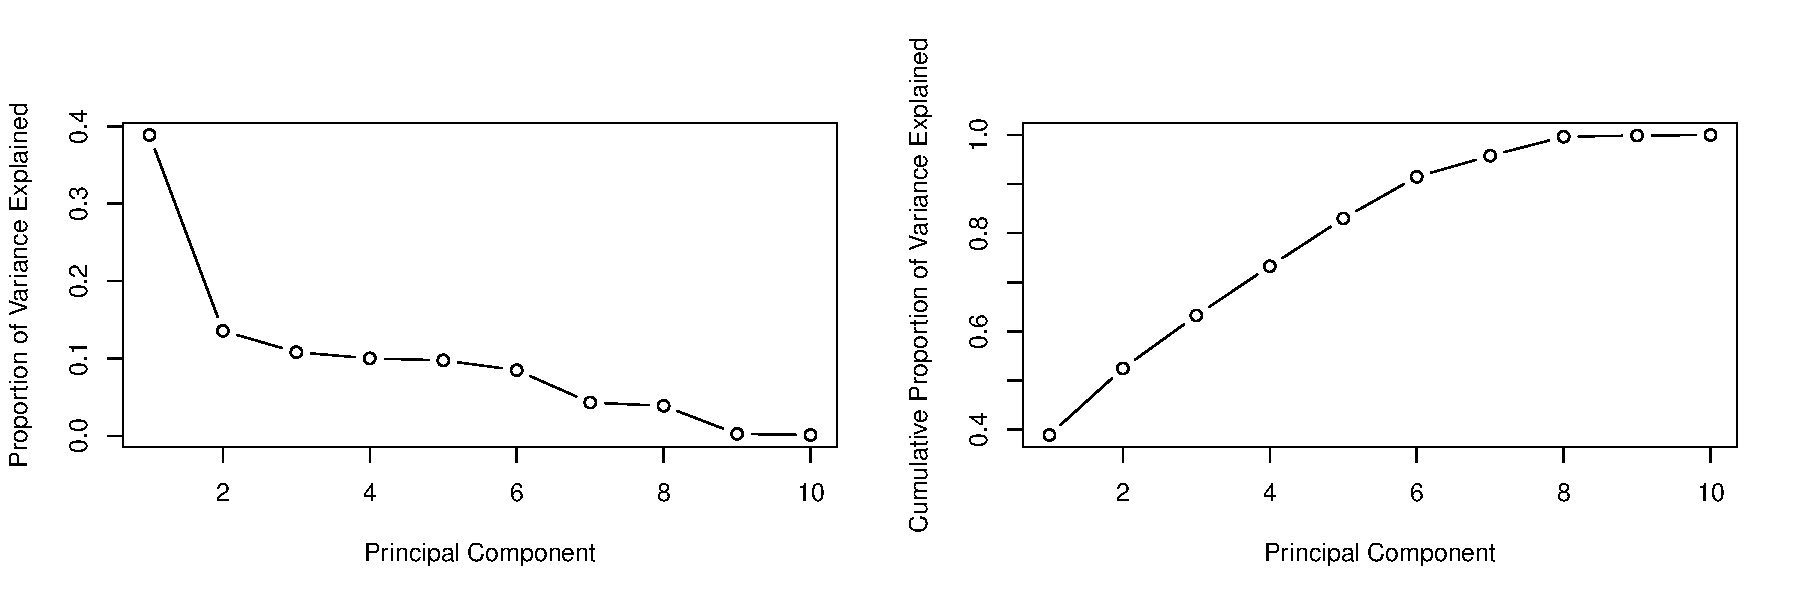
\includegraphics{deliverable_files/figure-latex/unnamed-chunk-10-1.pdf}

\begin{Shaded}
\begin{Highlighting}[]
\KeywordTok{par}\NormalTok{(op)}

\KeywordTok{summary}\NormalTok{(m2<-}\KeywordTok{lm}\NormalTok{(gross }\OperatorTok{~}\StringTok{ }\NormalTok{budget }\OperatorTok{+}\StringTok{ }\NormalTok{duration }\OperatorTok{+}\StringTok{ }\NormalTok{yearcat }\OperatorTok{+}\StringTok{ }\NormalTok{directorfl }\OperatorTok{+}\StringTok{ }\NormalTok{actor1fl }\OperatorTok{+}\StringTok{ }\NormalTok{actor2fl }\OperatorTok{+}\StringTok{ }\NormalTok{actor3fl }\OperatorTok{+}\StringTok{ }\NormalTok{castfl }\OperatorTok{+}\StringTok{ }\NormalTok{facenumber_in_poster }\OperatorTok{+}\StringTok{ }\NormalTok{genre, dataset))}
\end{Highlighting}
\end{Shaded}

\begin{verbatim}
## 
## Call:
## lm(formula = gross ~ budget + duration + yearcat + directorfl + 
##     actor1fl + actor2fl + actor3fl + castfl + facenumber_in_poster + 
##     genre, data = dataset)
## 
## Residuals:
##        Min         1Q     Median         3Q        Max 
## -189961474  -24134187   -6727230   16803034  481113705 
## 
## Coefficients:
##                        Estimate Std. Error t value Pr(>|t|)    
## (Intercept)          -5.665e+07  1.252e+07  -4.526 6.79e-06 ***
## budget                9.588e-01  5.831e-02  16.443  < 2e-16 ***
## duration              5.076e+05  1.058e+05   4.799 1.86e-06 ***
## yearcat2006-2010     -3.519e+05  3.946e+06  -0.089  0.92896    
## yearcat2011-2016     -1.098e+06  4.072e+06  -0.270  0.78750    
## directorfl            4.481e+02  5.580e+02   0.803  0.42214    
## actor1fl             -8.492e+03  1.442e+03  -5.887 5.50e-09 ***
## actor2fl             -8.430e+03  1.498e+03  -5.629 2.40e-08 ***
## actor3fl             -6.761e+03  2.411e+03  -2.804  0.00515 ** 
## castfl                8.478e+03  1.446e+03   5.863 6.30e-09 ***
## facenumber_in_poster -8.013e+05  7.046e+05  -1.137  0.25572    
## genreComedy           1.923e+07  7.611e+06   2.527  0.01167 *  
## genreDrama            4.161e+05  8.258e+06   0.050  0.95983    
## genreTerror           1.897e+07  8.660e+06   2.190  0.02874 *  
## ---
## Signif. codes:  0 '***' 0.001 '**' 0.01 '*' 0.05 '.' 0.1 ' ' 1
## 
## Residual standard error: 49700000 on 926 degrees of freedom
## Multiple R-squared:  0.5903, Adjusted R-squared:  0.5846 
## F-statistic: 102.7 on 13 and 926 DF,  p-value: < 2.2e-16
\end{verbatim}

\begin{Shaded}
\begin{Highlighting}[]
\NormalTok{op<-}\KeywordTok{par}\NormalTok{(}\DataTypeTok{mfrow=}\KeywordTok{c}\NormalTok{(}\DecValTok{2}\NormalTok{,}\DecValTok{2}\NormalTok{))}
\KeywordTok{plot}\NormalTok{(m2)}
\end{Highlighting}
\end{Shaded}

\includegraphics{deliverable_files/figure-latex/unnamed-chunk-10-2.pdf}

\begin{Shaded}
\begin{Highlighting}[]
\KeywordTok{par}\NormalTok{(op)}
\end{Highlighting}
\end{Shaded}

\subsection{Fitting the complete
model}\label{fitting-the-complete-model-1}

\begin{Shaded}
\begin{Highlighting}[]
\CommentTok{#step(m1, scope = list(lower=m1,upper=m2), direction="both", criterion = "BIC", k=log(940))}
\end{Highlighting}
\end{Shaded}


\end{document}
